\chapter{Auditory fMRI data \label{Chap:data:auditory}}
 
This experiment was conducted by Geraint Rees under the direction of Karl Friston and the FIL methods group. The purpose was to explore equipment and techniques in the early days of our fMRI experience. As such, it has not been formally written up, and is freely available for personal education and evaluation purposes.

This data set was the first ever collected and analysed in the Functional Imaging Laboratory (FIL) and is known locally as the mother of all experiments (MoAE).

This data set comprises whole brain BOLD/EPI images acquired on a modified 2T Siemens MAGNETOM Vision system. Each acquisition consisted of 64 contiguous slices (64$\times$64$\times$64 3$\times$3$\times$3 mm$^3$ voxels). Acquisition took 6.05s, with the scan to scan repeat time (TR) set arbitrarily to 7s.

96 acquisitions were made (TR=7s) from a single subject, in blocks of 6, giving 16 42s blocks. The condition for successive blocks alternated between rest and auditory stimulation, starting with rest. Auditory stimulation was bi-syllabic words presented binaurally at a rate of 60 per minute. The functional data starts at acquisition 4, image \texttt{fM00223\_004.\{hdr,img\}}, and are stored in folder \texttt{fM00223}. Due to T1 effects it is advisable to discard the first few scans (there were no ``dummy'' lead-in scans). A structural image was also acquired: \texttt{sM00223\_002.\{hdr,img\}}, stored in folder \texttt{sM00223}. These images are stored in Analyze format (now superseded by the NIfTI format, but SPM reads natively both formats and always saves images as NIfTI) and are available from the SPM site \footnote{Auditory fMRI dataset: \url{http://www.fil.ion.ucl.ac.uk/spm/data/auditory/}}.

To analyse the data, first create a new directory \texttt{DIR},  eg. \texttt{C:$\backslash$data$\backslash$auditory}, in which to place the results of your analysis. Then create 3 subdirectories (i) \texttt{dummy}, (ii) \texttt{jobs} and (iii) \texttt{classical}. As the analysis proceeds these directories will be filled with dummy scans, job-specification files, design matrices and models estimated using classical inference.
%and (iv) \texttt{bayesian} for Bayesian methods.

Start up \matlab\, enter your \texttt{jobs} directory and type \texttt{spm fmri} at the \matlab\ prompt. SPM will then open in fMRI mode with three windows (see Figure~\ref{aud_command}): (1) the top-left or ``Menu'' window, (2) the bottom-left or ``Interactive'' window and (3) the right-hand or ``Graphics'' window. Analysis then takes place in three major stages (i) spatial pre-processing, (ii) model specification, review and estimation and (iii) inference. These stages organise the buttons in SPM's Menu window.

\begin{figure}
\begin{center}
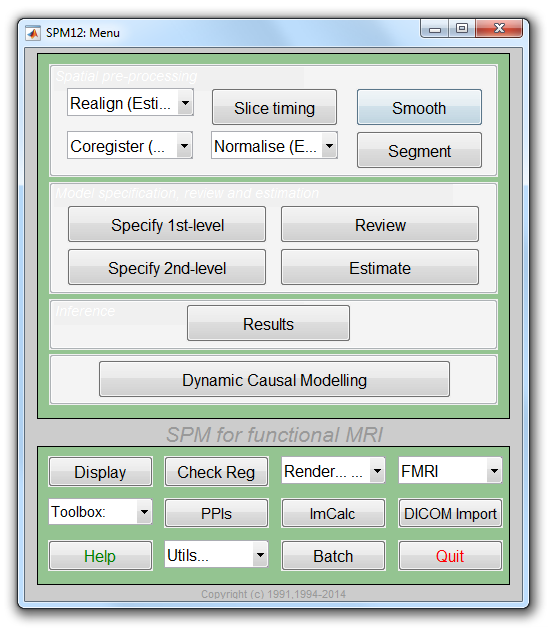
\includegraphics[width=100mm]{auditory/command}
\caption{\em The SPM base window comprises three sections i) spatial pre-processing, (ii) model specification, review and estimation and (iii) inference. \label{aud_command}}
\end{center}
\end{figure}

\section{Preamble (dummy scans)}

To avoid T1 effects in the initial scans of an fMRI time series we recommend discarding the first few scans. To make this example simple, we'll discard the first complete cycle (12 scans, \texttt{04-15}), leaving 84 scans, image files \texttt{16-99}. This is best done by moving these files to a different directory, \texttt{dummy}, that we created earlier.

\section{Spatial pre-processing}

\subsection{Realignment}

Under the spatial pre-processing section of the SPM Menu window select \textsc{Realign (Est \& Res)} from the \textsc{Realign} pulldown menu. This will call up a realignment job specification in the batch editor. Then
\begin{itemize}
\item Highlight ``Data'', select ``New Session'', then highlight the newly created ``Session'' option.
\item Press ``Select Files'' and use the SPM file selector to choose all of the functional images eg. (``\texttt{fM000*.img}''). There should be 84 files.
\item Press ``Resliced images'' in the ``Reslice Options'' and select ``Mean Image Only''.
\item Save the job file as eg. \texttt{DIR$\backslash$jobs$\backslash$realign.mat}.
\item Press the \texttt{RUN} button in the batch editor (green arrow).
\end{itemize}

This will run the realign job which will estimate the 6 parameter (rigid body) spatial transformation that will align the times series of images and will modify the header of the input images (\texttt{*.hdr}), such that they reflect the relative orientation of the data after correction for movement artefacts. SPM will then plot the estimated time series of translations and rotations shown in Figure~\ref{aud_realign}. These data are also saved to a file eg. \texttt{rp\_fM00223\_016.txt}, so that these variables can be later used as regressors when fitting GLMs. This allows movements effects to be discounted when looking for brain activations.

SPM will also create a mean image eg. \texttt{meanfM00223\_016.img} which will be used in the next step of spatial processing - coregistration.

\begin{figure}
\begin{center}
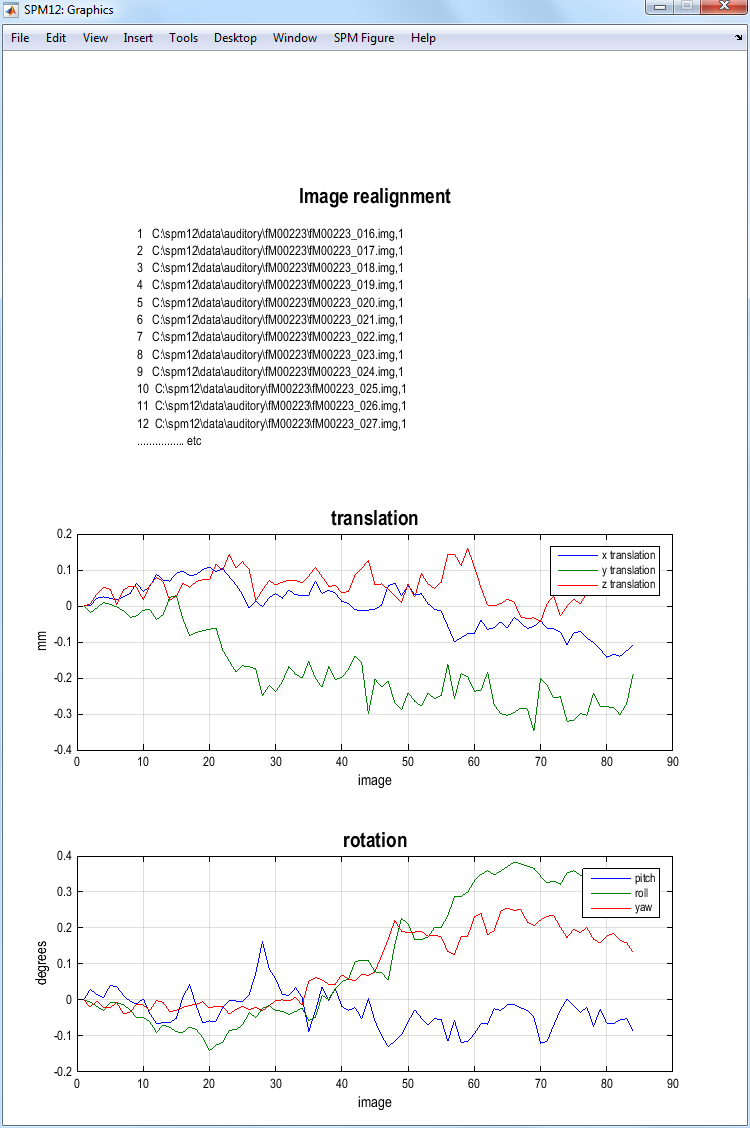
\includegraphics[width=125mm]{auditory/realign}
\caption{\em Realignment of Auditory data.\label{aud_realign}}
\end{center}
\end{figure}

\subsection{Coregistration}

Select \textsc{Coregister (Estimate)} from the \textsc{Coregister} pulldown. This will call up the specification of a coregistration job in the batch editor. 

\begin{itemize}
\item Highlight ``Reference Image'' and then select the mean fMRI scan from realignment eg. \texttt{meanfM00223\_016.img}.
\item Highlight ``Source Image'' and then select the structural image eg. \texttt{sM00223\_002.img}.
\item Press the Save button and save the job as \texttt{DIR$\backslash$jobs$\backslash$coregister.mat}.
\item Then press the \texttt{RUN} button.
\end{itemize}

SPM will then implement a coregistration between the structural and functional data that maximises the mutual information. The image in figure~\ref{aud_coreg} should then appear in the Graphics window. SPM will have changed the header of the source file which in this case is the structural image \texttt{sM00223\_002.hdr}.
\begin{figure}
\begin{center}
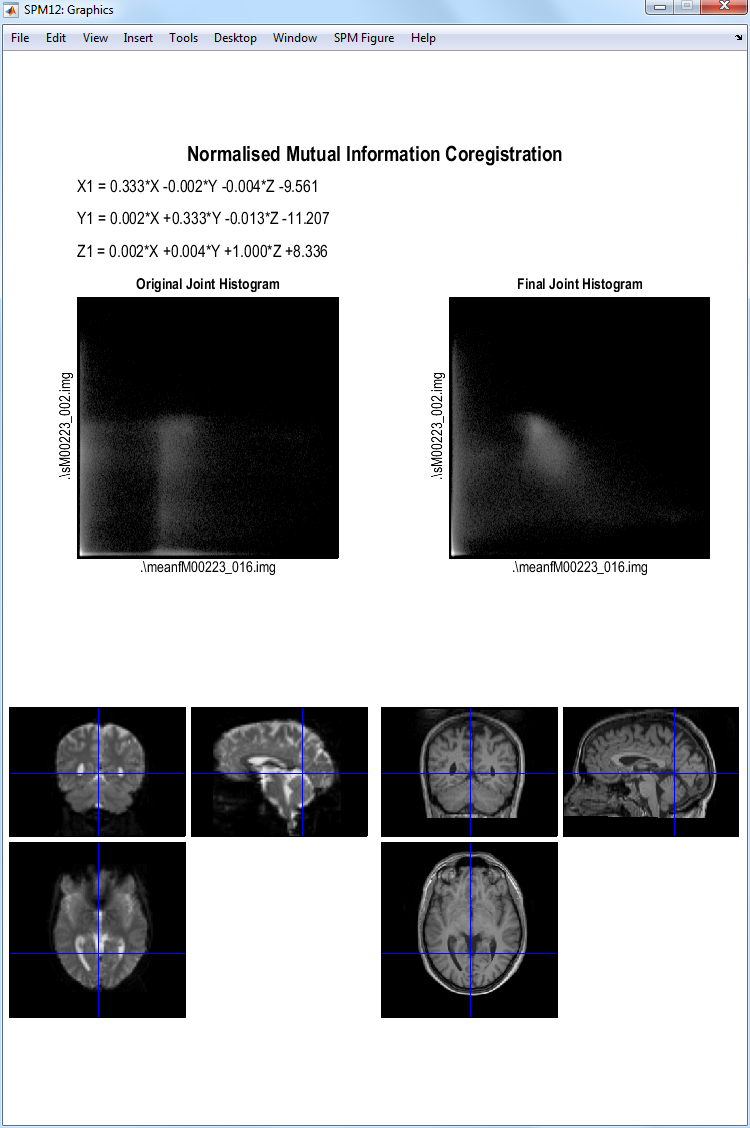
\includegraphics[width=125mm]{auditory/coreg}
\caption{\em Mutual Information Coregistration of Auditory data.\label{aud_coreg}}
\end{center}
\end{figure}

The \textsc{Check Reg} facility is useful here, to check the results of coregistration. Press the \textsc{Check Reg} button in the lower section of the Menu window and then select the ``Reference'' and ``Source'' Images specified above ie \texttt{meanfM00223\_016.img} and \texttt{sM00223\_002.img}. SPM will then produce an image like that shown in Figure~\ref{aud_checkreg} in the Graphics window. You can then use your mouse to navigate these images to confirm that there is an anatomical correspondence.

\begin{figure}
\begin{center}
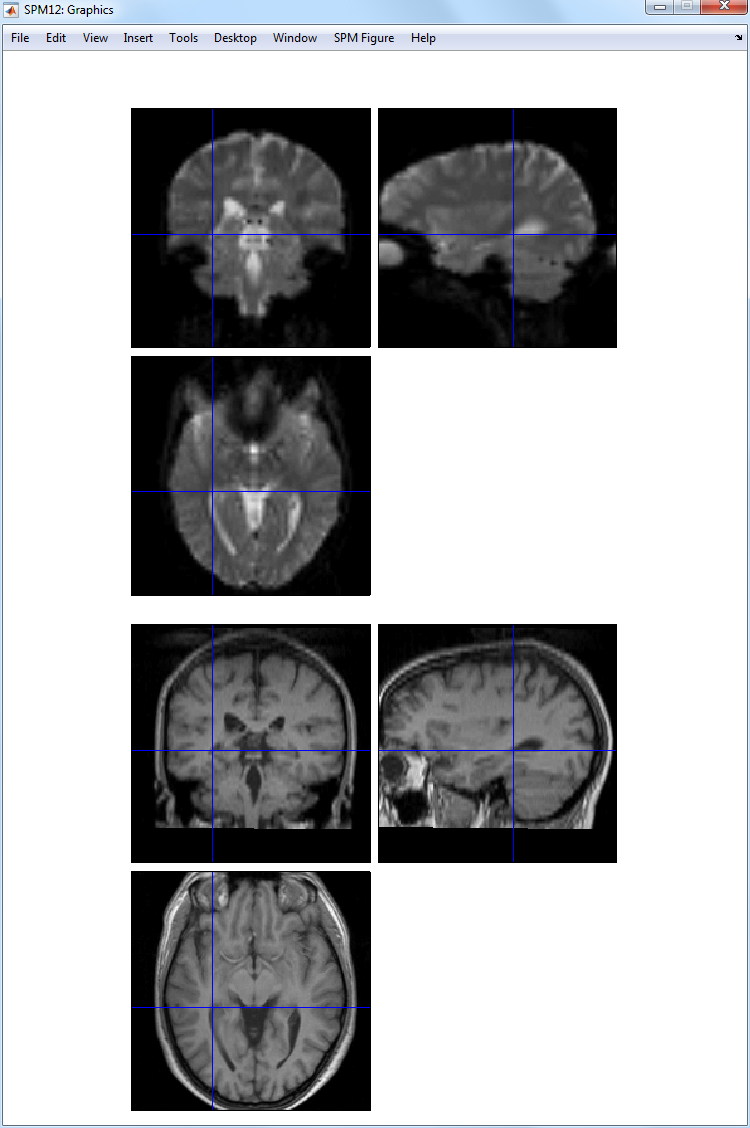
\includegraphics[width=125mm]{auditory/checkreg}
\caption{\em Checking registration of functional and ``registered'' structural data. \label{aud_checkreg}}
\end{center}
\end{figure}

\subsection{Segmentation}

Press the \textsc{Segment} button. This will call up the specification of a segmentation job in the batch editor. Highlight the ``Volumes'' field and then select the subject's registered anatomical image eg. \texttt{sM00223\_002.img}. Highlight ``Save Bias Corrected'' and select ``Save Bias Corrected''. Highlight ``Deformation Fields'' \t the bottom of the list and select ``Forward''. Save the job file as \texttt{segment.mat} and then press \texttt{RUN}. SPM will segment the structural image using the default tissue probability maps as priors. 

SPM will create gray and white matter images and bias-field corrected structural image. These can be viewed using the \textsc{CheckReg} facility as described in the previous section. Figure~\ref{aud_gray} shows the gray matter image, \texttt{c1sM0023\_002.nii} along with the original structural. Figure~\ref{aud_bias} shows the structural and bias-corrected image, \texttt{msM0023\_002.nii}.

\begin{figure}
\begin{center}
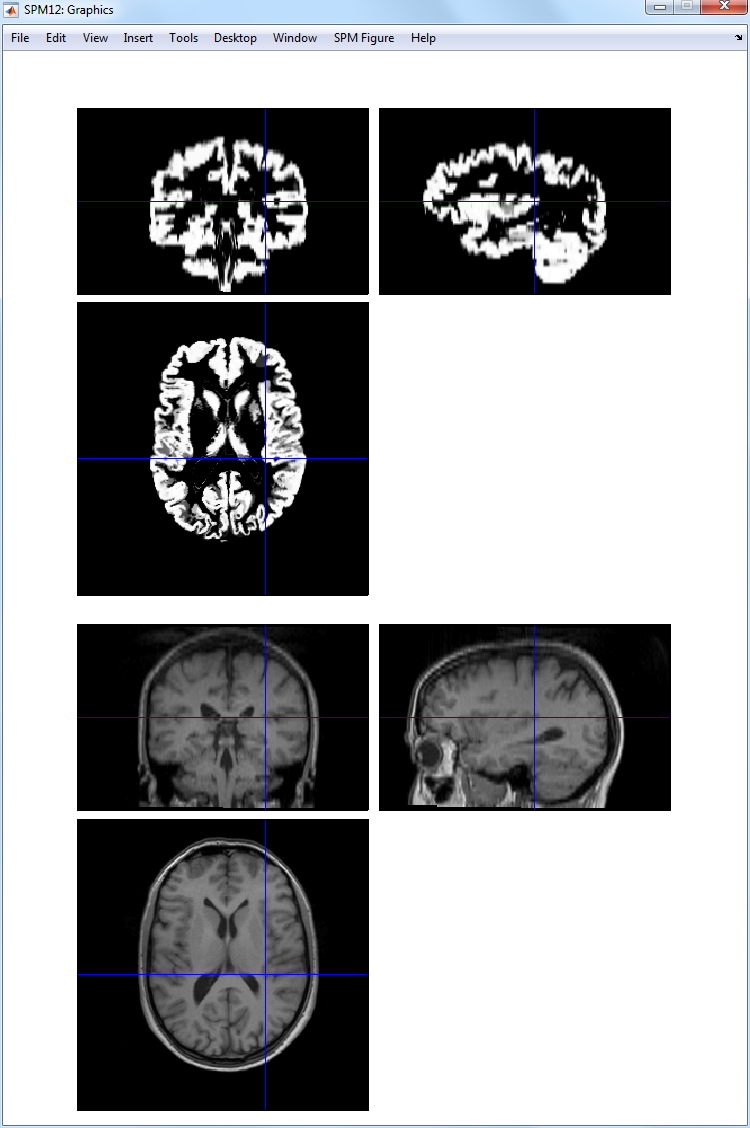
\includegraphics[width=125mm]{auditory/gray}
\caption{\em Gray matter image and ``registered'' structural image.\label{aud_gray}}
\end{center}
\end{figure}

\begin{figure}
\begin{center}
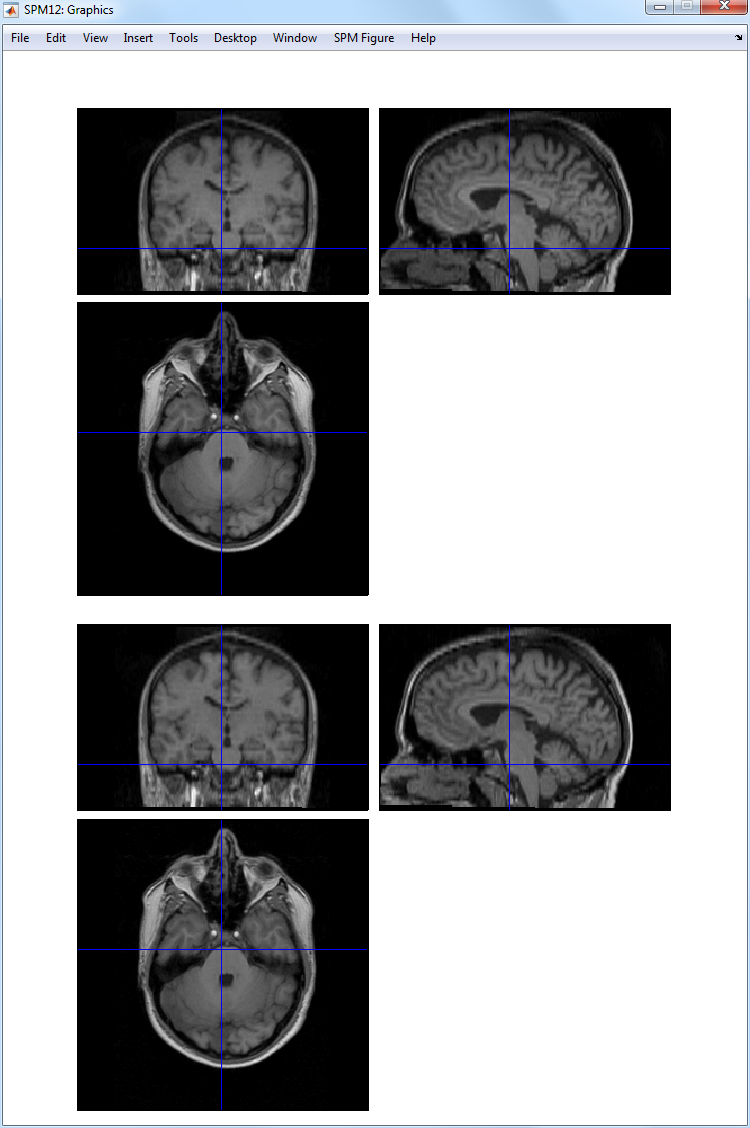
\includegraphics[width=125mm]{auditory/bias}
\caption{\em Structural image (top) and bias-corrected structural image (bottom). Notice that the original structural is darker at the top than at the bottom. This non-uniformity has been removed in the bias-corrected image.\label{aud_bias}}
\end{center}
\end{figure}

SPM will also write a deformation field, file \texttt{y\_sM00223\_002.nii} in the original structural directory. It contains 3 volumes to encode the x, y and z coordinates. Given that the structural and functional data are in alignment, this can be used to spatially normalise the functional data. 

\subsection{Normalise}

Select \textsc{Normalise (Write)} from the \textsc{Normalise} pulldown menu. This will call up the specification of a normalise job in the batch editor. 

\begin{itemize}
\item Highlight ``Data'', select New ``Subject'',
\item Highlight ``Deformation Field'' and select the \texttt{y\_sM00223\_002.nii} file that you created in the previous section,
\item Highlight ``Images to Write'' and select all of the realigned functional images \texttt{fM000*.img}. You can right click over the listed files, choose ``Select all'' and press ``Done''.
\item In the ``Writing Options'', change ``Voxel sizes'' from [2 2 2] to [3 3 3]. This step is not strictly necessary: it will write images out at a resolution closer to that at which they were acquired.
%\footnote{This will speed up subsequent analysis and is necessary, for example, to make Bayesian fMRI analysis computationally efficient.}
\item Press ``Save'', save the job as \texttt{normalise\_functional.mat} and then press the \texttt{RUN} button.
\end{itemize}

SPM will then write spatially normalised files to the functional data directory. These files have the prefix \texttt{w}.

If you wish to superimpose a subject's functional activations on their own anatomy\footnote{Beginners may wish to skip this step, and instead just superimpose functional activations on an ``average structural image''.} you will also need to apply the spatial normalisation parameters to their (bias-corrected) anatomical image. To do this

\begin{itemize}
\item Select \textsc{Normalise (Write)}, highlight ``Data'', select ``New Subject''.
\item Highlight ``Deformation Field'', select the  \texttt{y\_sM00223\_002.nii} file that you created in the previous section, press ``Done''.
\item Highlight ``Images to Write'', select the bias-corrected structural eg. \texttt{msM00223\_002.nii}, press ``Done''.
\item Open ``Writing Options'', select voxel sizes and change the default [2 2 2] to [1 1 3] which corresponds to the original resolution of the images.
\item Save the job as \texttt{normalise\_structural.mat} and press the \texttt{RUN} button.
\end{itemize}

\subsection{Smoothing}

Press the \textsc{Smooth} button. This will call up the specification of a smooth job in the batch editor.
%\footnote{The smoothing step is unnecessary if you are only interested in Bayesian analysis of your functional data.}

\begin{itemize}
\item Select ``Images to Smooth'' and then select the spatially normalised files created in the last section eg. \texttt{wf*.img}. This can be done efficiently by changing the filter in the SPM file selector to \texttt{\textasciicircum wf.*}. SPM will then only list those files beginning with letters \texttt{wf} ie. those that have been spatially normalised.
\item Highlight ``FWHM'' and change [8 8 8] to [6 6 6]. This will smooth the data by 6mm in each direction.
\item Save the job as \texttt{smooth.mat} and press the \texttt{Run} button.
\end{itemize}

An example of functional image and its smoothed version is displayed on Figure~\ref{aud_smooth}.

\begin{figure}
\begin{center}
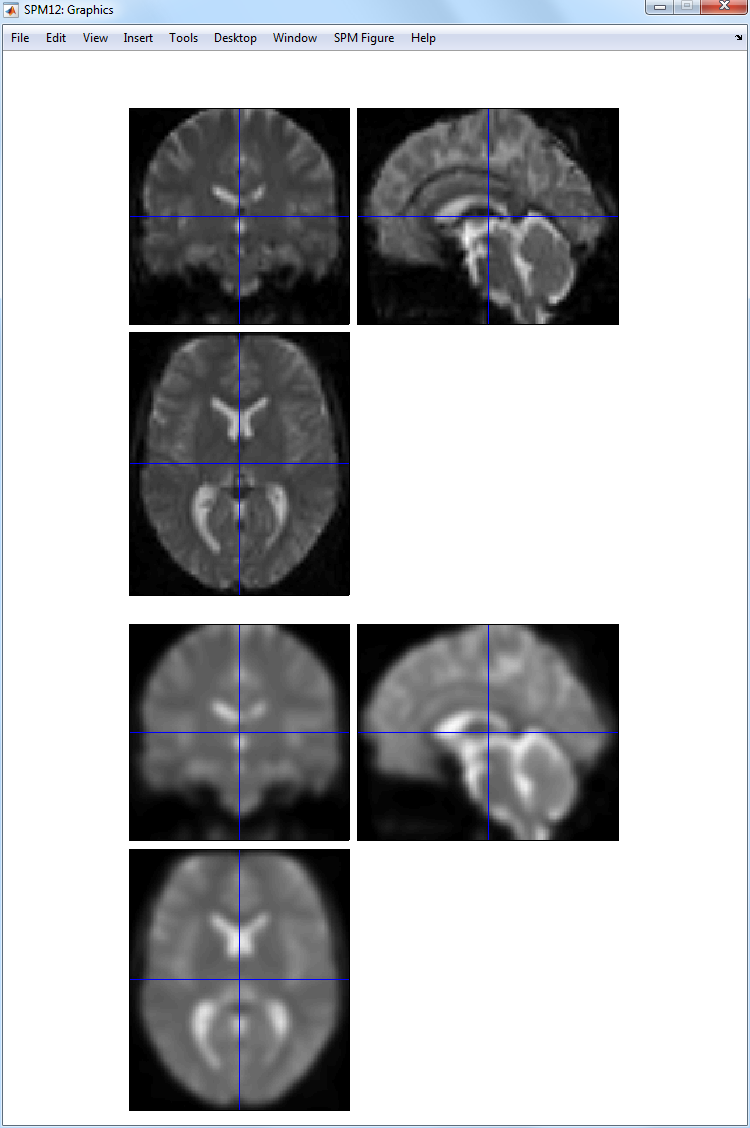
\includegraphics[width=125mm]{auditory/smooth}
\caption{\em Functional image (top) and 6mm-smoothed functional image (bottom). These images were obtained using SPM's ``CheckReg'' facility. \label{aud_smooth}}
\end{center}
\end{figure}

\section{Model specification, review and estimation}

Press the ``Specify 1st-level'' button. This will call up the specification of an fMRI specification job in the batch editor. Then

\begin{itemize}
\item Open the ``Timing parameters'' option.
\item Highlight ``Units for design'' and select ``Scans''.
\item Highlight ``Interscan interval'' and enter 7. That's the TR in seconds.
\item Highlight ``Data and Design'' and select ``New Subject/Session''. Then open the newly created ``Subject/Session'' option.
\item Highlight ``Scans'' and use SPM's file selector to choose the 84 smoothed, normalised functional images ie \texttt{swfM00223\_016.img} to \texttt{swfM00223\_099.img}. These can be selected easily using the \texttt{\textasciicircum sw.*'} filter, and select all. Then press ``Done''.
\item Highlight ``Condition'' and select ``New condition''.
\item Open the newly created ``Condition'' option. Highlight ``Name'' and enter ``listening''. Highlight ``Onsets'' and enter ``6:12:84''. Highlight ``Durations'' and enter ``6''.
\item Highlight ``Directory'' and select the \texttt{DIR/classical} directory you created earlier.
\item Save the job as \texttt{specify.mat} and press the \texttt{Run} button.
\end{itemize}

SPM will then write an \texttt{SPM.mat} file to the \texttt{DIR/classical} directory. It will also plot the design matrix, as shown in Figure~\ref{aud_design}. 

\begin{figure}
\begin{center}
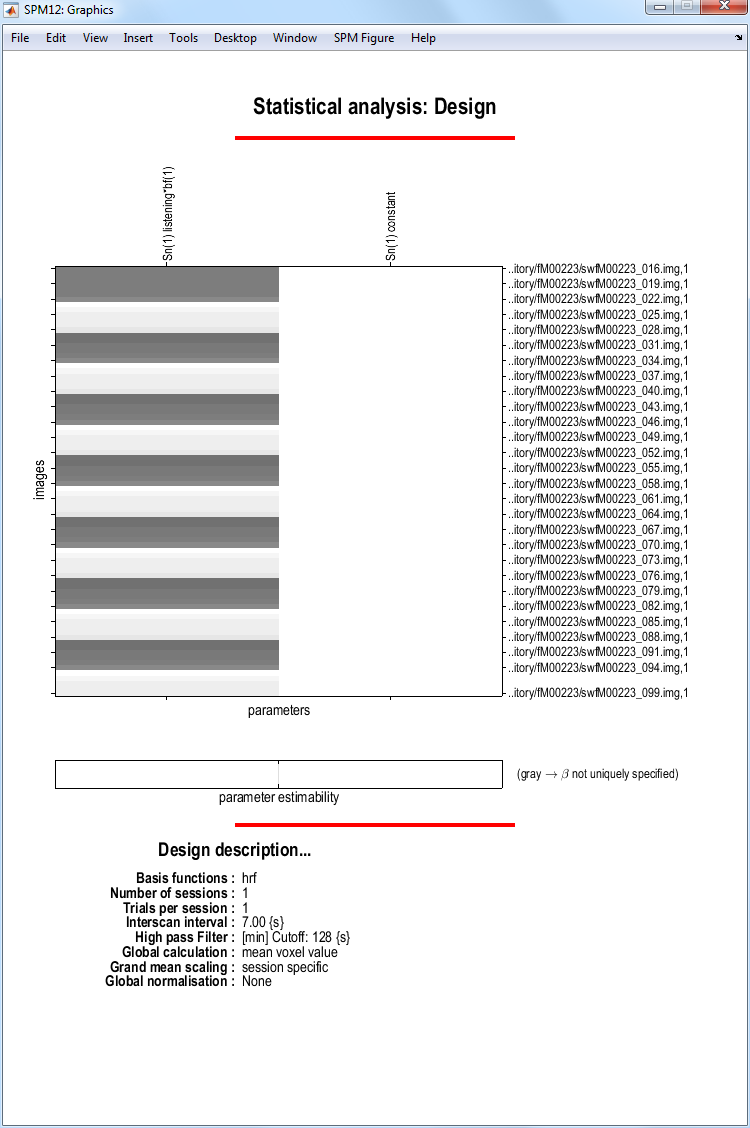
\includegraphics[width=125mm]{auditory/design}
\caption{\emph{\texttt{Design matrix}: The filenames on the right-hand side of the design matrix indicate the scan associated with each row.\label{aud_design}}}
\end{center}
\end{figure}

At this stage it is advisable to check your model specification using SPM's review facility which is accessed via the ``Review'' button. This brings up a ``design'' tab on the interactive window clicking on which produces a pulldown menu. If you select the first item ``Design Matrix'' SPM will produce the image shown in Figure~\ref{aud_design}. If you select ``Explore'' then ``Session 1'' then ``listening'', SPM will produce the plots shown in Figure~\ref{aud_explore}.

\begin{figure}
\begin{center}
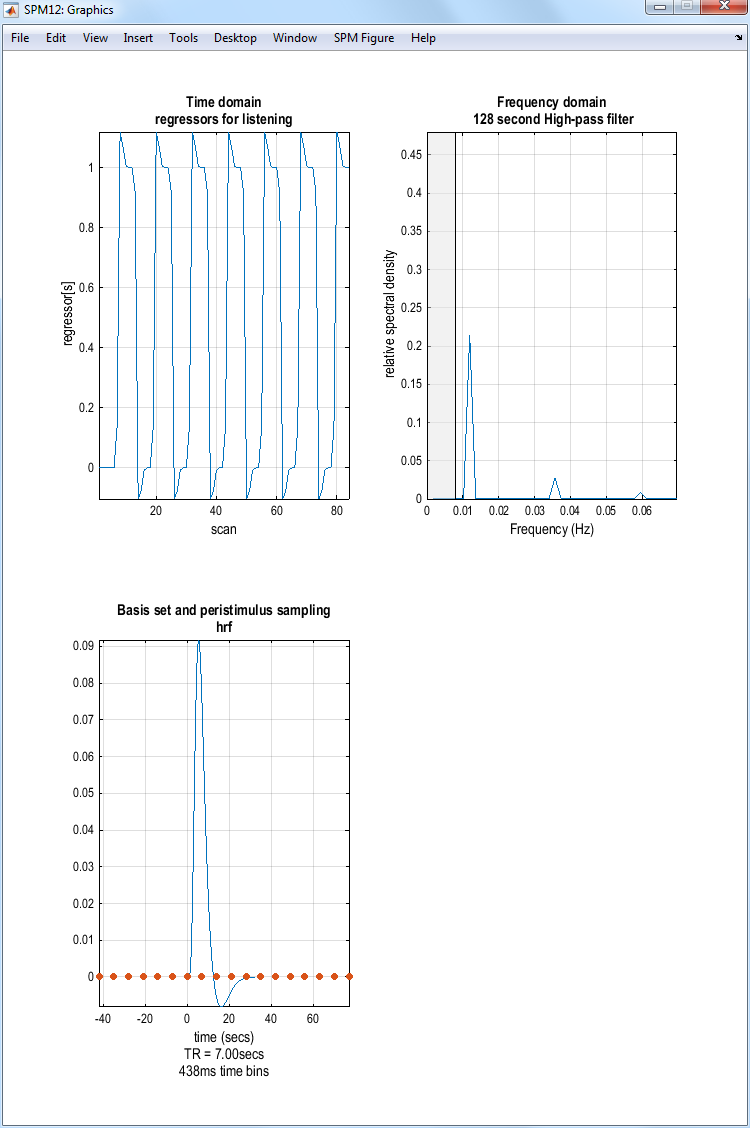
\includegraphics[width=125mm]{auditory/explore}
\caption{\emph{\texttt{Exploring the design matrix in Figure~\ref{aud_design}}: This shows the time series of the ``listening'' regressor (top left), a frequency domain plot of the ``listening'' regressor (top right) and the basis function used to convert assumed neuronal activity into hemodynamic activity. In this model we used the default option - the canonical basis function. The frequency domain plot shows that the frequency content of the ``listening'' regressor is above the set frequencies that are removed by the High Pass Filter (HPF) (these are shown in gray - in this model we accepted the default HPF cut-off of 128s or 0.008Hz). \label{aud_explore}}}
\end{center}
\end{figure}

If you select the second item on the ``Design'' tab, ``Design Orthogonality'', SPM will produce the plot shown in Figure~\ref{aud_orth}. Columns $x_1$ and $x_2$ are orthogonal if the inner product $x_1^T x_2=0$. The inner product can also be written $x_1^T x_2 = |x_1||x_2| cos \theta$ where $|x|$ denotes the length of $x$ and $\theta$ is the angle between the two vectors. So, the vectors will be orthogonal if $cos \theta=0$. The upper-diagonal elements in the matrix at the bottom of figure~\ref{aud_orth} plot $cos\theta$ for each pair of columns in the design matrix. Here we have a single entry.  A degree of non-orthogonality or collinearity is indicated by the gray shading.

\begin{figure}
\begin{center}
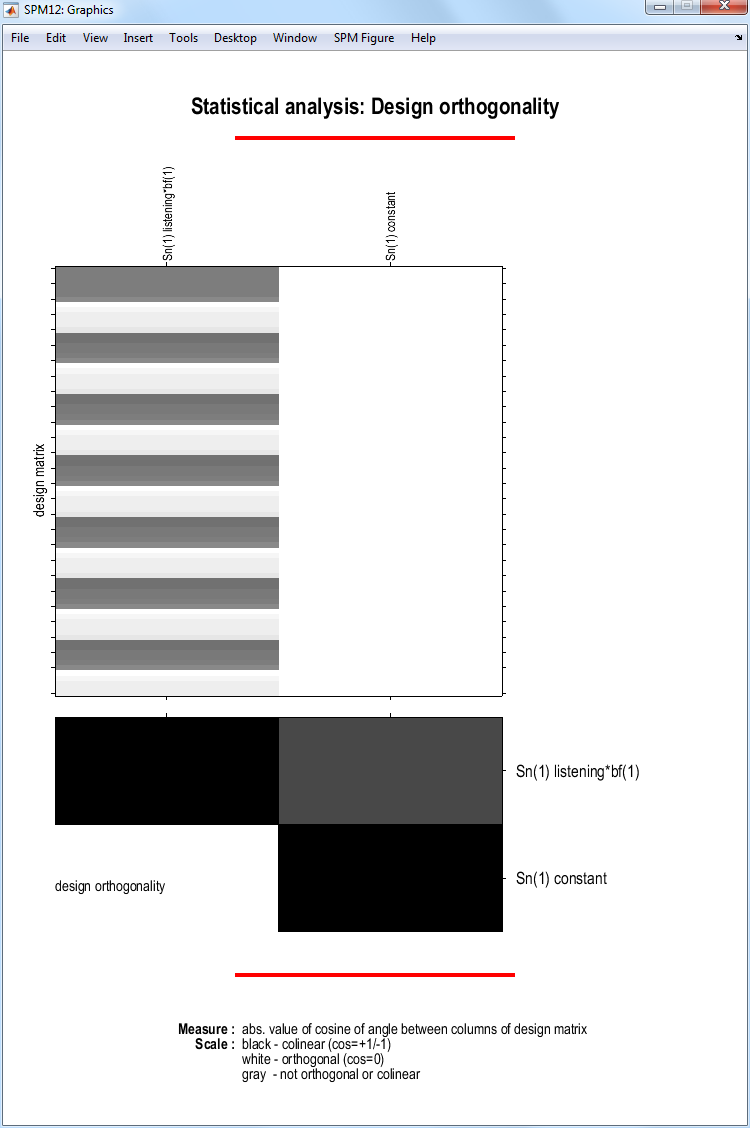
\includegraphics[width=80mm]{auditory/aud_orth}
\caption{\emph{\texttt{Design Orthogonality}: The description above the first column in the design matrix {\sf Sn(1)Listening*bf(1)} means that this column refers to the first session of data (in this analysis there is only 1 session), the name of this condition/trial is `listening' and the trial information has been convolved with the first basis function (the canonical hemodynamic response). The constant regressor for session 1 is referred to as {\sf Sn(1)Constant}. The orthogonality matrix at the bottom indicates a degree of collinearity between regressors. \label{aud_orth}}}
\end{center}
\end{figure}

\subsection{Estimate}

Press the \textsc{Estimate} button. This will call up the specification of an fMRI estimation job in the batch editor. Then

\begin{itemize}
\item Highlight the ``Select SPM.mat'' option and then choose the \texttt{SPM.mat} file saved in the \texttt{classical} subdirectory.
\item Save the job as \texttt{estimate.mat} and press the \texttt{Run} button.
\end{itemize}

SPM will write a number of files into the selected directory including an \texttt{SPM.mat} file.

\section{Inference}

After estimation:

\begin{itemize}
\item Press ``Results''.
\item Select the \texttt{SPM.mat} file created in the last section.
\end{itemize}

\begin{figure}
\begin{center}
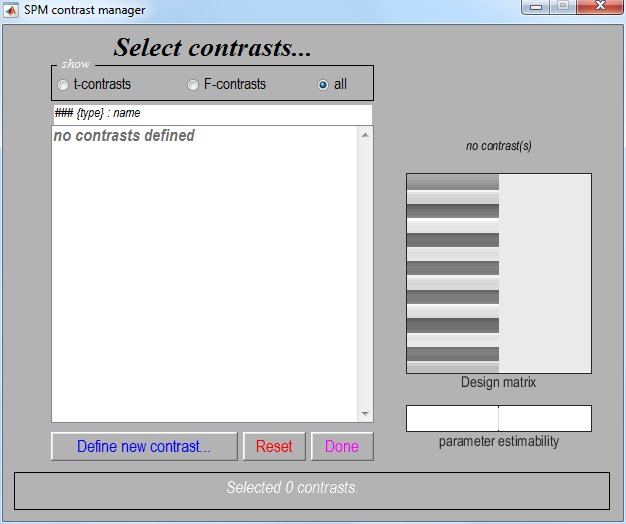
\includegraphics[width=75mm]{auditory/con_man}
\caption{\emph{The contrast manager}}
\end{center}
\end{figure}

This will invoke the contrast manager.

\subsection{Contrast manager}

The contrast manager displays the design matrix (surfable) in the right panel and lists specified contrasts in the left panel. Either ``t-contrast'' or ``F-contrast'' can be selected. To examine statistical results for condition effects

\begin{itemize}
\item{Select ``Define new contrast''}
\end{itemize}
\begin{figure}
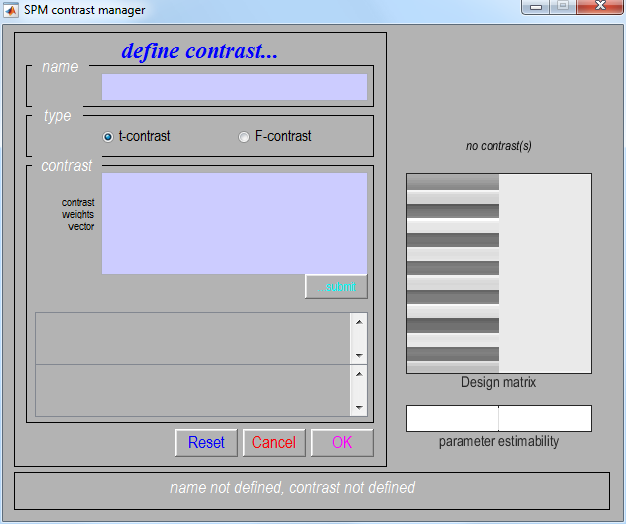
\includegraphics[width=75mm]{auditory/con_man2}
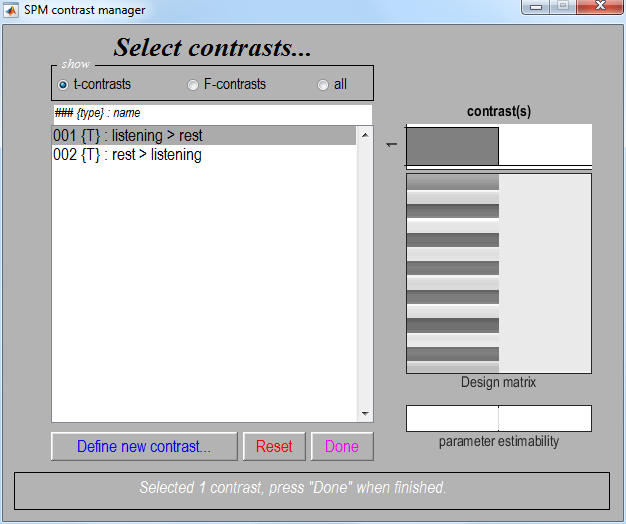
\includegraphics[width=75mm]{auditory/con_man3}
\caption{\emph{Left: A contrast is entered by specifying the numeric values in the lower window and the name in the upper window. Right: After contrasts have been specified they can be selected.}}
\end{figure}

One sided main effects for the listening condition (i.e., a one-sided t-test) can be specified (in this example) as ``1'' (listening $>$ rest) and ``-1'' (rest $>$ listening). SPM will accept estimable contrasts only. Accepted contrasts are displayed at the bottom of the contrast manager window in green, incorrect ones are displayed in red. To view a contrast

\begin{itemize}
\item Select the contrast name e.g., ``listening $>$ rest''.
\item Press ``Done''.
\end{itemize}

\subsection{Masking}

You will then be prompted with

\begin{itemize}
\item  \emph{Apply masking ? [none/contrast/image]}.
\item ``Specify none''.
\end{itemize}

Masking implies selecting voxels specified by other contrasts. If ``yes'', SPM will prompt for (one or more) masking contrasts, the significance level of the mask (default \textit{p} = 0.05 uncorrected), and will ask whether an inclusive or exclusive mask should be used. Exclusive will remove all voxels which reach the default level of significance in the masking contrast, inclusive will remove all voxels which do not reach the default level of significance in the masking contrast. Masking does not affect \textit{p}-values of the ``target'' contrast, it only includes or excludes voxels.

\subsection{Thresholds}

You will then be prompted with

\begin{itemize}
\item \emph{p value adjustment to control: [FWE/none]}.
\begin{itemize}
\item Select ``FWE''.
\end{itemize}
\item \emph{p value(family-wise error)}.
\begin{itemize}
\item Accept the default value, 0.05.
\end{itemize}
\end{itemize}

A Family Wise Error (FWE) is a false positive anywhere in the SPM. Now, imagine repeating your experiment many times and producing SPMs. The proportion of SPMs containing FWEs is the FWE rate. A value of 0.05 implies that on average 1 in 20 SPMs contains one or more false positives somewhere in the image. 

If you choose the ``none'' option above this corresponds to making statistical inferences at the ``voxel level''. These use ``uncorrected'' \textit{p} values, whereas FWE thresholds are said to use ``corrected'' \textit{p}-values. SPM's default uncorrected \textit{p}-value is \textit{p}=0.001. This means that the probability of a false positive at each voxel is 0.001. So if, you have 50,000 voxels you can expect $50,000 \times 0.001 = 50$ false positives in each SPM.

%The final option here is False Discovery Rate (FDR). If you set this at 0.1, this means that of all the discoveries you make (ie. above threshold voxels that appear in the SPM) 10\% of them are likely to be false. 

You will then be prompted with

\begin{itemize}
\item \emph{Extent Threshold \{voxels\} [0]}.
\begin{itemize}
\item Accept the default value, ``0''.
\end{itemize}
\end{itemize}

Entering a value $k$ here will produce SPMs with clusters containing at least $k$ voxels. SPM will then produce the SPM shown in Figure~\ref{aud_spm1}.

\begin{figure}
\begin{center}
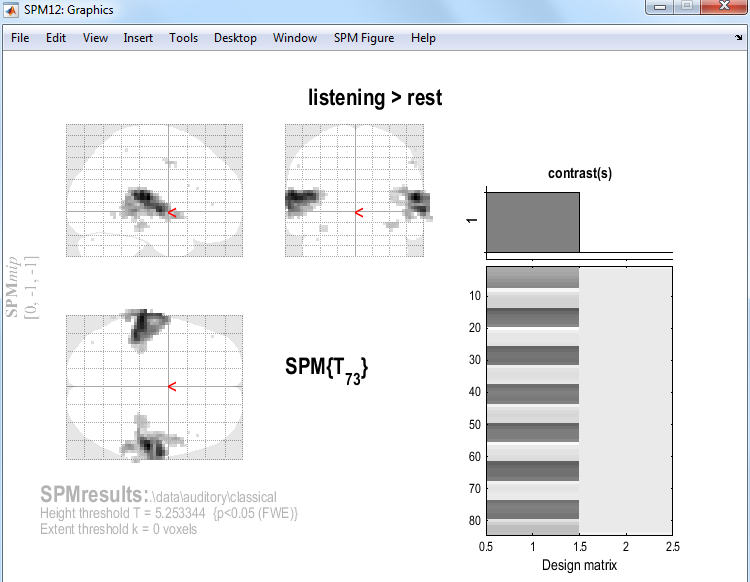
\includegraphics[width=100mm]{auditory/spm1}
\caption{\em SPM showing bilateral activation of auditory cortex. \label{aud_spm1}}
\end{center}
\end{figure}

\subsection{Files}

A number of files are written to the working directory at this time.
Images containing weighted parameter estimates are saved as \texttt{con\_0001.nii}, \texttt{con\_0002.nii}, etc. in the working directory. Images of T-statistics are saved as \texttt{spmT\_0001.nii}, \texttt{spmT\_0002.nii} etc., also in the working directory.

\subsection{Maximum Intensity Projections}

SPM displays a Maximum Intensity Projection (MIP) of the statistical map in the Graphics window. The MIP is projected on a glass brain in three orthogonal planes. The MIP is surfable: right-clicking in the MIP will activate a pulldown menu, left-clicking  on the red cursor will allow it to be dragged to a new position.

\begin{figure}
\begin{center}
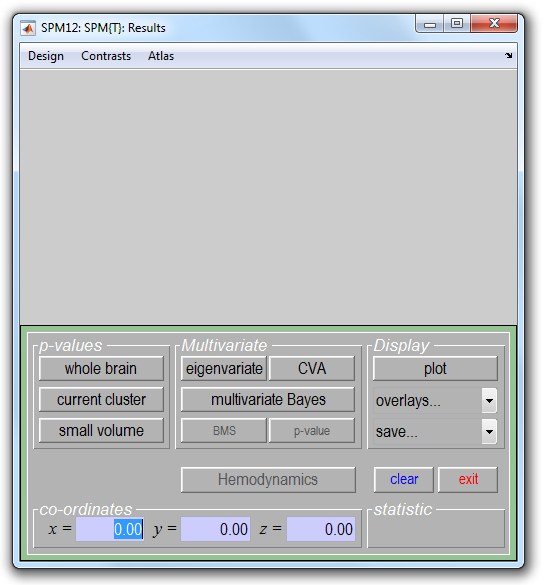
\includegraphics[width=100mm]{auditory/interactive}
\caption{\em SPM's Interactive window during results assessment. The ``\textit{p}-values'' section is used to produce tables of statistical information. The visualisation section is used to plot responses at a voxel or to visual activations overlaid on anatomical images. The ``Multivariate'' section, ie. the ``eigenvariate'' button, is used to extract data for subsequent analyses such as assessment of PsychoPhysiological Interactions (PPIs) or Dynamic  Causal Models (DCMs).}
\end{center}
\end{figure}

\subsection{Design matrix}

SPM also displays the design matrix with the selected contrast. The design matrix is also surfable: right-clicking will show parameter names, left-clicking will show design matrix values for each scan. 

In the SPM Interactive window (lower left panel) a button box appears with various options for displaying statistical results (p-values panel) and creating plots/overlays (visualisation panel). Clicking ``Design'' (upper left) will activate a pulldown menu as in the ``Explore design'' option.

\subsection{Statistical tables}

To get a summary of local maxima, press the ``whole brain'' button in the \textit{p}-values section of the Interactive window. This will list all clusters above the chosen level of significance as well as separate ($>$8mm apart) maxima within a cluster, with details of significance thresholds and search volume underneath, as shown in Figure~\ref{aud_volume}

\begin{figure}
\begin{center}
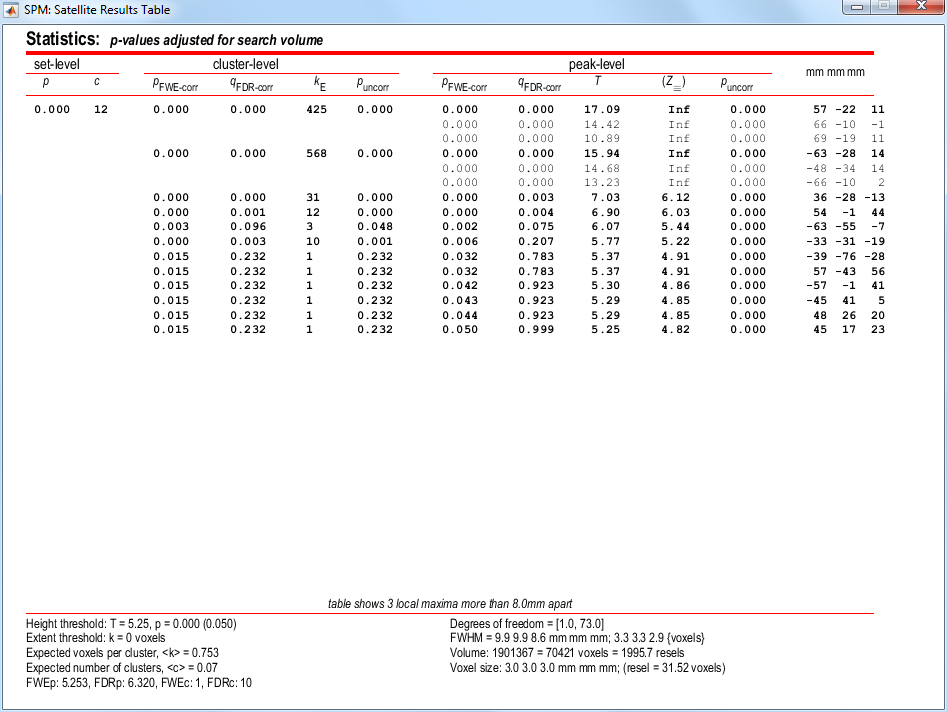
\includegraphics[width=100mm]{auditory/volume}
\caption{\em Volume table for ``listening $>$ rest'' effect. This table of values was created by pressing the SPM Figure $>$ Results Table option at the top of the Graphics window and then pressing the ``whole brain'' button. This displays the table of results in a separate window. \label{aud_volume}}
\end{center}
\end{figure}

The columns in volume table show, from right to left:

\begin{itemize}
\item \textbf{x, y, z (mm)}: coordinates in MNI space for each maximum.
\item \textbf{peak-level}: the chance (\textit{p}) of finding (under the null hypothesis) a peak with this or a greater height (T- or Z-statistic), corrected (FWE or FDR)/ uncorrected for search volume.
\item \textbf{cluster-level}: the chance (\textit{p}) of finding a cluster with this many (\textit{k}) or a greater number of voxels, corrected (FWE or FDR)/ uncorrected for search volume.
\item \textbf{set-level}: the chance (\textit{p}) of finding this (\textit{c}) or a greater number of clusters in the search volume.
\end{itemize}

It is also worth noting that:

\begin{itemize}
\item The table is surfable: clicking a row of cluster coordinates will move the pointer in the MIP to that cluster, clicking other numbers will display the exact value in the \matlab\ window (e.g. 0.000 = 6.1971e-07).
\item To inspect a specific cluster (e.g., in this example data set, the right auditory cortex), either move the cursor in the MIP (by left-clicking and dragging the cursor, or right-clicking the MIP background which will activate a pulldown menu).
\item Alternatively, click the cluster coordinates in the volume table, or type the coordinates in the co-ordinates section of the Interactive window.
\end{itemize}

It is also possible to produce tables of statistical information for a single cluster of interest rather than for the whole volume. Firstly, select the relevant cluster in the MIP and then press the ``current cluster'' button in the \textit{p}-values section of the Interactive window. This will show coordinates and voxel-level statistics for local maxima ($>$4mm apart) in the selected cluster. This table is also surfable.

\subsection{Plotting responses at a voxel}

A voxel can be chosen with coordinates corresponding to those in the Interactive window. The responses at this voxel can then be plotted using the ``Plot'' button in the visualisation section of the Interactive window. This will provide you with five further options:

\begin{enumerate}
\item Contrast estimates and 90\% CI: SPM will prompt for a specific contrast (e.g., listening$>$rest). The plot will show effect size and 90\% confidence intervals. See eg. Figure~\ref{aud_contrast}.
\item Fitted responses: Plots adjusted data and fitted response across session/subject. SPM will prompt for a specific contrast and provides the option to choose different ordinates (``an explanatory variable'', ``scan or time'', or ``user specified''). If ``scan or time'', the plot will show adjusted or fitted data with errors added as shown in Figure~\ref{aud_fitted}.
\item Event-related responses: Plots adjusted data and fitted response across peri-stimulus time.
\item Parametric responses.
\item Volterra kernels.
\end{enumerate}

\begin{figure}
\begin{center}
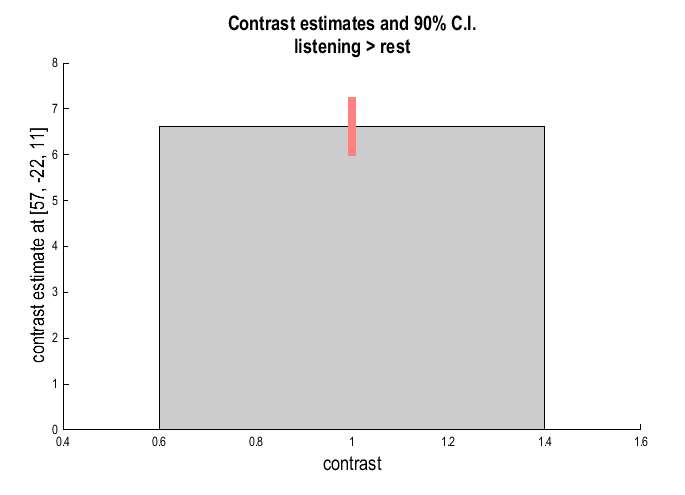
\includegraphics[width=60mm]{auditory/contrast}
\caption{\em Estimated effect size. \label{aud_contrast}}
\end{center}
\end{figure}

\begin{figure}
\begin{center}
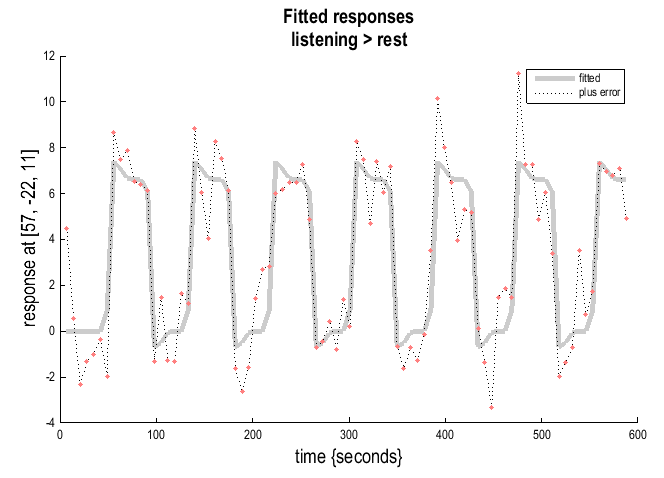
\includegraphics[width=60mm]{auditory/fitted}
\caption{\em Fitted responses. \label{aud_fitted}}
\end{center}
\end{figure}

For plotting event-related responses SPM provides three options

\begin{enumerate}
\item Fitted response and PSTH (peri-stimulus time histogram): plots mean regressor(s) (ie. averaged over session) and mean signal +/- SE for each peri-stimulus time bin.
\item Fitted response and 90\% CI: plots mean regressor(s) along with a 90\% confidence interval.
\item Fitted response and adjusted data: plots regressor(s) and individual data (note that in this example the data are shown in columns due to the fixed TR/ISI relationship).
\end{enumerate}

Its worth noting that

\begin{itemize}
\item The values for the fitted response across session/subject for the selected plot can be displayed and accessed in the \matlab window by typing ``Y''. Typing ``y'' will display the adjusted data.
\item ``Adjusted'' data = adjusted for confounds (e.g., global flow) and high- and low pass filtering.
\end{itemize}

\subsection{Overlays}

The visualisation section of the Interactive window also provides an overlay facility for anatomical visualisation of clusters of activation. Pressing ``Overlays'' will activate a pulldown menu with several options including:

\begin{enumerate}
\item \textbf{Slices}: overlay on three adjacent (2mm) transaxial slices. SPM will prompt for an image for rendering. This could be a canonical image (see \texttt{spm\_templates.man}) or an individual T1/mean EPI image for single-subject analyses. Beware that the left-right convention in the display of that option will depend on how your data are actually stored on disk.
\item \textbf{Sections}: overlay on three intersecting (sagittal, coronal, axial) slices. These renderings are surfable: clicking the images will move the crosshair.
\item \textbf{Render}: overlay on a volume rendered brain.
\end{enumerate}

Thresholded SPMs can be saved as NIfTI image files in the working directory by using the ``Save'' button in the Interactive window. In Figures~\ref{aud_slices}, \ref{aud_sections} and \ref{aud_render} the `listening $>$ rest' activation has been superimposed on the spatially normalised, bias-corrected anatomical image \texttt{wmsM00223\_002.nii} created earlier. 

\begin{figure}
\begin{center}
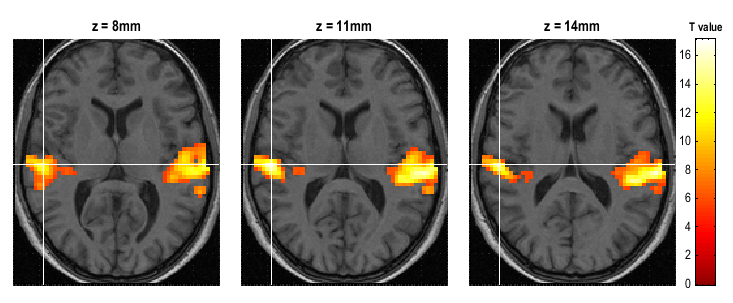
\includegraphics[width=100mm]{auditory/slices}
\caption{\emph{Slices.} \label{aud_slices} }
\end{center}
\end{figure}

\begin{figure}
\begin{center}
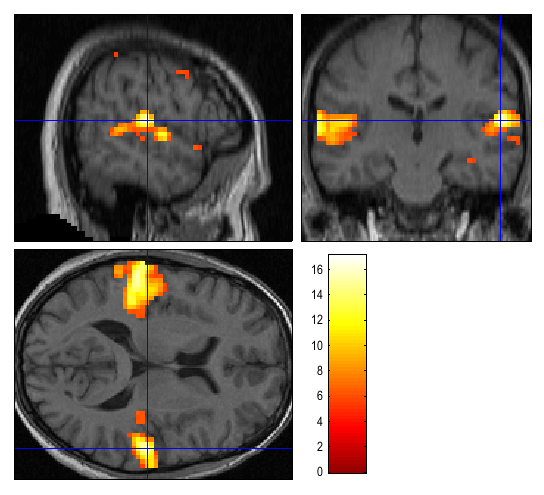
\includegraphics[width=100mm]{auditory/sections}
\caption{\emph{Sections.} \label{aud_sections} }
\end{center}
\end{figure}

For the ``Render'' option we first created a rendering for this subject. This was implemented by 

\begin{itemize}
\item ``Normalise (Write)'' the two images \texttt{c1sM00223\_002.nii} and \texttt{c2sM00223\_002.nii} using the ``Deformation Field'' \texttt{y\_sM00223\_002.nii} and a voxel size of [1 1 1].
\item Selecting ``Extract Surface'' from the ``Render'' pulldown menu.
\item Selecting the gray and white matter images \texttt{wc1sM00223\_002.nii} and \texttt{wc2sM00223\_002.nii} created in the first step.
\item Saving the results using the default options (Rendering and Surface).
\end{itemize}

SPM plots the rendered anatomical image in the graphics window and saves it as \texttt{render\_\-wc1sM00223\_\-002.mat}. The surface image is saved as \texttt{surf\_wc1sM00223\_002.mat}.

\begin{figure}
\begin{center}
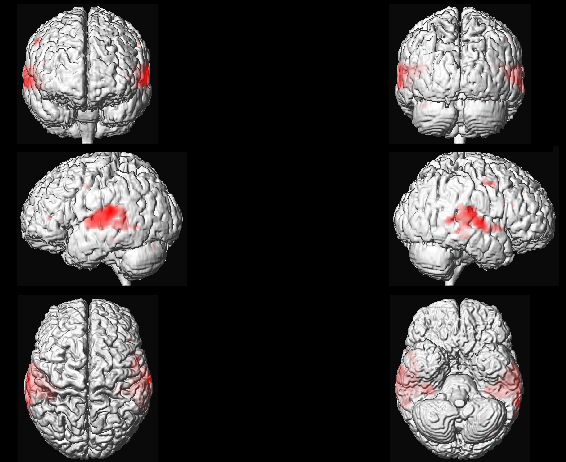
\includegraphics[width=100mm]{auditory/render}
\caption{\emph{Render.} \label{aud_render} }
\end{center}
\end{figure}

It is also possible to project and display the results on a surface mesh, we are going to use here one of the canonical mesh distributed with SPM (in MNI space). Press ``Overlays'' and choose ``Render'', then go in the \texttt{canonical} folder of your SPM installation and select file \texttt{cortex\_20484.surf.gii} (this is a surface mesh stored using the GIfTI format) and you will obtain a figure similar to \ref{aud_render2}.

\begin{figure}
\begin{center}
\includemovie[
	poster,
	toolbar,
    label=Render,
    text=Render (Acrobat Reader required),
    3Droo=300,
    3Dcoo=0 -22.5 17.5,
    3Dc2c=1 0 0,
    3Daac=30,
    3Droll=0,
    3Dlights=Day,
    3Dbg=0 0 0,
]{\linewidth}{100mm}{auditory/render.u3d}
\caption{\emph{3D Rendering using canonical mesh.} \label{aud_render2}}
\end{center}
\end{figure}

%\subsection{Miscellaneous}
%
%Other options (in the results controls panel):
%
%\begin{itemize}
%\item \textbf{clear}: clears lower subpanel of Graphics window,
%\item \textbf{exit}: exits the results section,
%\item \textbf{?}: launches help.
%\end{itemize}

%\section{Bayesian analysis}
%
%\subsection{Specification}
%
%Press the ``Specify 1st-level'' button. This will call up an fMRI specification job in the batch editor. Then
%
%\begin{itemize}
%\item Open the fMRI model specification option.
%\item Load the ``specify.mat'' job file created for the classical analysis.
%\item Open ``Subject/Session'', highlight ``Scans''.
%\item Deselect the smoothed functional images using the ``unselect all'' option available from a right mouse click in the SPM file selector (bottom window).
%\item Select the unsmoothed functional images using the \texttt{\textasciicircum w.*} filter and `select all' option available from a right mouse click in the SPM file selector (top right window)\footnote{Remember not to select the first 12 scans, scans 4 to 15, as these may contain T1 effects. This can be done during selection or by first moving the files to a different directory.}. The Bayesian analysis uses a spatial prior where the spatial regularity in the signal is estimated from the data. It is therefore not necessary to create smoothed images if you are only going to do a Bayesian analysis.
%\item Press ``Done''.
%\item Highlight ``Directory'' and select the \texttt{DIR/bayesian} directory you created earlier (you will first need to deselect the \texttt{DIR/classical} directory).
%\item Save the job as \texttt{specify\_bayesian.mat} and press the ``Run'' button.
%\end{itemize}
%
%\subsection{Estimation}
%
%Press the ``Estimate'' button. This will call up the specification of an fMRI estimation job in the batch editor. Then
%
%\begin{itemize}
%\item Highlight the ``Select SPM.mat'' option and then choose the SPM.mat file saved in the \texttt{DIR/bayesian} directory.
%\item Highlight ``Method'' and select the ``Choose Bayesian 1st-level'' option.
%\item Open the newly created ``Bayesian 1st-level'' option, highlight ``AR model order'' and select 0. This data set has a TR=7s, so is unlikely to have temporally autocorrelated errors.
%\item Save the job as \texttt{estimate\_bayesian.job} and press the ``Run'' butto.
%\end{itemize}
%
%SPM will write a number of files into the output directory including 
%
%\begin{itemize}
%\item An \texttt{SPM.mat} file.
%\item Images of estimated regression coefficients  \texttt{Cbeta\_0001.nii} and \texttt{Cbeta\_0002.nii}. These filenames are prefixed with a \texttt{C} indicating that these are the mean values of the ``Conditional'' or ``Posterior'' density.
%\item Images of error bars/standard deviations on the regression coefficients \texttt{SDbeta\_0001.nii} and \texttt{SDbeta\_0002.nii}.
%\item An image of the standard deviation of the error \texttt{Sess1\_SDerror.nii}.
%\item An image \texttt{mask.nii} indicating which voxels were included in the analysis.
%\end{itemize}
%
%\subsection{Inference}
%
%After estimation:
%
%\begin{itemize}
%\item Press ``Results'',
%\item Select the \texttt{SPM.mat} file created in the last section,
%\item Select ``Define new contrast'',
%\item Enter the name ``active $>$ rest'',
%\item Enter the value ``1'', press ``Submit'', ``OK'', ``Done'',
%\item \emph{Mask with other contrast ? [Yes/No]},
%\item Specify No,
%\item Title for comparison, accept the default,
%\item \emph{Effect size threshold for PPM},
%\item Enter the value 2,
%\item \emph{Posterior probability threshold for PPM},
%\item Enter the value 0.99,
%\item \emph{Extent threshold [0]},
%\item Accept the default value,
%\item \emph{Plot effect size [Yes/No]},
%\item Select the default `Yes'.
%\end{itemize}
%
%SPM will then plot a map of effect sizes at voxels where it is 99\% sure that the effect size is greater than 2\% of the global mean. This is a large activation. Then use overlays, sections, select the normalised structural image created earlier and move the cursor to the activation in the left hemisphere. This should create the plot shown in Figure~\ref{aud_bayes}.
%
%\begin{figure}
%\begin{center}
%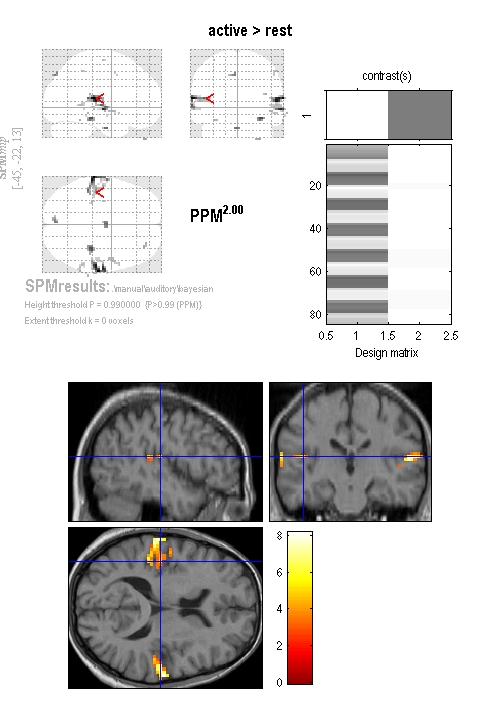
\includegraphics[width=100mm]{auditory/aud_bayes}
%\caption{\em \textbf{Bayesian analysis:} MIP and overlay of effect sizes at voxels where SPM is 99\% sure that the effect size is greater than 2\% of the global mean. \label{aud_bayes} }
%\end{center}
%\end{figure}
%
%It is also possible to look for regions where responses in the active condition are different to those at rest. Active responses could be greater or smaller.
%
%\begin{itemize}
%\item Press ``Results'',
%\item Select the \texttt{SPM.mat} file created in the last section,
%\item Select ``Define new contrast'' and highlight the ``F'' radio button,
%\item Enter the name ``active != rest'',
%\item Enter the value ``1'', press ``Submit'', ``OK'', ``Done'',
%\item \emph{Mask with other contrast ? [Yes/No]},
%\item Specify ``No'',
%\item Title for comparison, accept the default,
%\item \emph{Posterior probability threshold for PPM},
%\item Accept the default value\footnote{The default PPM threshold is set to $1-1/S$ where S is the number of voxels in the volume being analysed. The rationale for this is that inference is based on an approximate posterior distribution, $Q$, which factorises across voxels. The approximate posterior is chosen to best match the true posterior in the sense of KL-divergence. Given the factorisation in $Q$, the expected number of false positives in the PPM is 1. },
%\item \emph{Extent threshold [0]},
%\item Accept the default value, 0,
%\item \emph{Plot effect size [Yes/No]},
%\item Select the default ``Yes''.
%\end{itemize}
%
%SPM will then plot a map of $\chi^2$ statistic values at above threshold voxels. Then use overlays, sections, select the normalised structural image created earlier and move the cursor to the activation in the left hemisphere. This should create the plot shown in Figure~\ref{aud_bayes2}
%
%\begin{figure}
%\begin{center}
%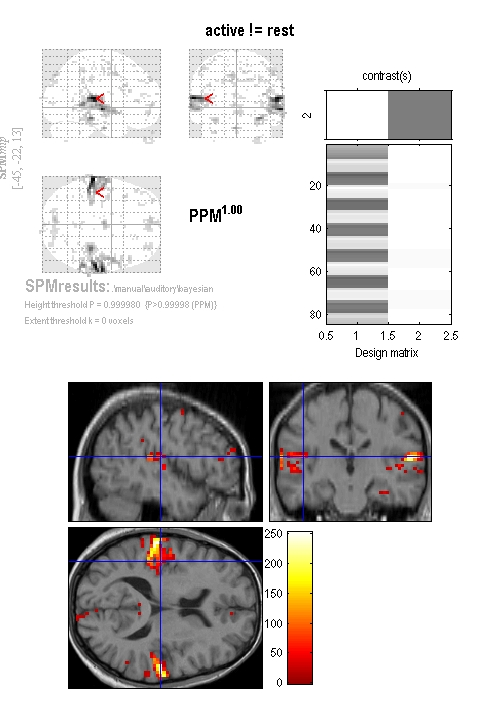
\includegraphics[width=100mm]{auditory/aud_bayes2}
%\caption{\em \textbf{Two-sided Bayesian analysis:} MIP and overlay of $\chi^2$ statistic values at above threshold voxels. This shows regions where activity is different between active and rest conditions, whether positive or negative. \label{aud_bayes2} }
%\end{center}
%\end{figure}
%
%When you revisit the contrast manager this contrast will be referred to as a ``P'' contrast, rather than an ``F'' contrast. This indicates that Bayes rule is used to make the inference. To indicate that we are testing a two-sided effect it is advisable to make this clear when naming the contrast (as we have done with the label ``active != rest'').

